%!TEX program = xelatex

\documentclass[compress]{beamer}
%--------------------------------------------------------------------------
% Common packages
%--------------------------------------------------------------------------

\definecolor{links}{HTML}{663000}
\hypersetup{colorlinks,linkcolor=,urlcolor=links}

\usepackage[english]{babel}
\usepackage{pgfpages} % required for notes on second screen
\usepackage{graphicx}

\usepackage{multicol}

\usepackage{tabularx,ragged2e}
\usepackage{booktabs}

\setlength{\emergencystretch}{3em}  % prevent overfull lines
\providecommand{\tightlist}{%
  \setlength{\itemsep}{0pt}\setlength{\parskip}{0pt}}


\usetheme{hri}

% Display the navigation bullet even without subsections
\usepackage{remreset}% tiny package containing just the \@removefromreset command
\makeatletter
\@removefromreset{subsection}{section}
\makeatother
\setcounter{subsection}{1}

\makeatletter
\let\beamer@writeslidentry@miniframeson=\beamer@writeslidentry
\def\beamer@writeslidentry@miniframesoff{%
  \expandafter\beamer@ifempty\expandafter{\beamer@framestartpage}{}% does not happen normally
  {%else
    % removed \addtocontents commands
    \clearpage\beamer@notesactions%
  }
}
\newcommand*{\miniframeson}{\let\beamer@writeslidentry=\beamer@writeslidentry@miniframeson}
\newcommand*{\miniframesoff}{\let\beamer@writeslidentry=\beamer@writeslidentry@miniframesoff}
\makeatother



\newcommand{\source}[2]{{\tiny\it Source: \href{#1}{#2}}}

\usepackage{tikz}
\usetikzlibrary{mindmap,backgrounds,positioning,calc,patterns}
\usepackage{pgfplots}
\pgfplotsset{compat=newest}
\usepackage{circuitikz}

\graphicspath{{figs/}}

\title{ROCO222 \newline Intro to Sensors and Actuators}
\subtitle{Electromagnetism \& DC motor -- Part 1}

\date{}
\author{Séverin Lemaignan}
\institute{Centre for Robotics and Neural Systems\\{\bf Plymouth University}}

\begin{document}


%%%%%%%%%%%%%%%%%%%%%%%%%%%%%%%%%%%%%%%%%%%%%%%%%%%%%%%%

\licenseframe{github.com/severin-lemaignan/module-introduction-sensors-actuators}

%%%%%%%%%%%%%%%%%%%%%%%%%%%%%%%%%%%%%%%%%%%%%%%%%%%%%%%%

\maketitle

%%%%%%%%%%%%%%%%%%%%%%%%%%%%%%%%%%%%%%%%%%%%%%%%%%%%%%%%

\section{Electromagnetism}

%%%%%%%%%%%%%%%%%%%%%%%%%%%%%%%%%%%%%%%%%%%%%%%%%%%%%%%%

{\fullbackground[scale=0.9,page=2]{ian-electromagnetism.pdf}
    \begin{frame}{Lines of field from a bar magnet}
    \end{frame}
}

%%%%%%%%%%%%%%%%%%%%%%%%%%%%%%%%%%%%%%%%%%%%%%%%%%%%%%%%

    \begin{frame}{Like poles repel and unlike poles attract}
    \end{frame}

%%%%%%%%%%%%%%%%%%%%%%%%%%%%%%%%%%%%%%%%%%%%%%%%%%%%%%%%

{\fullbackground[scale=0.9,page=4]{ian-electromagnetism.pdf}
    \begin{frame}{Like poles repel and unlike poles attract}
    \end{frame}
}


%%%%%%%%%%%%%%%%%%%%%%%%%%%%%%%%%%%%%%%%%%%%%%%%%%%%%%%%

{\fullbackground[scale=0.9,page=7]{ian-electromagnetism.pdf}
    \begin{frame}{Solenoid and bar magnets have similar lines of field}
    \end{frame}
}

%%%%%%%%%%%%%%%%%%%%%%%%%%%%%%%%%%%%%%%%%%%%%%%%%%%%%%%%

{\fullbackground[scale=0.9,page=8]{ian-electromagnetism.pdf}
    \begin{frame}{Direction of conventional current}
    \end{frame}
}

%%%%%%%%%%%%%%%%%%%%%%%%%%%%%%%%%%%%%%%%%%%%%%%%%%%%%%%%

{\fullbackground[scale=0.9,page=9]{ian-electromagnetism.pdf}
    \begin{frame}{Magnetic field strength H and flux density B}
    \end{frame}
}

%%%%%%%%%%%%%%%%%%%%%%%%%%%%%%%%%%%%%%%%%%%%%%%%%%%%%%%%

{\fullbackground[scale=0.9,page=10]{ian-electromagnetism.pdf}
    \begin{frame}{FIeld around a current carrying wire}
    \end{frame}
}

%%%%%%%%%%%%%%%%%%%%%%%%%%%%%%%%%%%%%%%%%%%%%%%%%%%%%%%%

{\fullbackground[scale=0.9,page=11]{ian-electromagnetism.pdf}
    \begin{frame}{The direction of induced magnetic field}
    \end{frame}
}

%%%%%%%%%%%%%%%%%%%%%%%%%%%%%%%%%%%%%%%%%%%%%%%%%%%%%%%%

{\fullbackground[scale=0.9,page=12]{ian-electromagnetism.pdf}
    \begin{frame}{The direction of induced magnetic field}
    \end{frame}
}

%%%%%%%%%%%%%%%%%%%%%%%%%%%%%%%%%%%%%%%%%%%%%%%%%%%%%%%%

{\fullbackground[scale=0.9,page=13]{ian-electromagnetism.pdf}
    \begin{frame}{Iron filings can show field around wire}
    \end{frame}
}

%%%%%%%%%%%%%%%%%%%%%%%%%%%%%%%%%%%%%%%%%%%%%%%%%%%%%%%%
\miniframesoff
{\fullbackground[scale=0.9,page=14]{ian-electromagnetism.pdf}
    \begin{frame}{Iron filings can show field around wire}
    \end{frame}
}
\miniframeson

%%%%%%%%%%%%%%%%%%%%%%%%%%%%%%%%%%%%%%%%%%%%%%%%%%%%%%%%

{\fullbackground[scale=0.9,page=15]{ian-electromagnetism.pdf}
    \begin{frame}{Flux of magnetic field}
    \end{frame}
}

%%%%%%%%%%%%%%%%%%%%%%%%%%%%%%%%%%%%%%%%%%%%%%%%%%%%%%%%

{\fullbackground[scale=0.9,page=16]{ian-electromagnetism.pdf}
    \begin{frame}{Ampere's law}
    \end{frame}
}

%%%%%%%%%%%%%%%%%%%%%%%%%%%%%%%%%%%%%%%%%%%%%%%%%%%%%%%%

{\fullbackground[scale=0.9,page=17]{ian-electromagnetism.pdf}
    \begin{frame}{Ampere's law}
    \end{frame}
}

%%%%%%%%%%%%%%%%%%%%%%%%%%%%%%%%%%%%%%%%%%%%%%%%%%%%%%%%

{\fullbackground[scale=0.9,page=18]{ian-electromagnetism.pdf}
    \begin{frame}{Simple example of Ampere's law}
    \end{frame}
}

%%%%%%%%%%%%%%%%%%%%%%%%%%%%%%%%%%%%%%%%%%%%%%%%%%%%%%%%
\miniframesoff
{\fullbackground[scale=0.9,page=19]{ian-electromagnetism.pdf}
    \begin{frame}{Simple example of Ampere's law}
    \end{frame}
}
\miniframeson

%%%%%%%%%%%%%%%%%%%%%%%%%%%%%%%%%%%%%%%%%%%%%%%%%%%%%%%%

{\fullbackground[scale=0.9,page=20]{ian-electromagnetism.pdf}
    \begin{frame}{Ampere's law for current in straight wire}
    \end{frame}
}

%%%%%%%%%%%%%%%%%%%%%%%%%%%%%%%%%%%%%%%%%%%%%%%%%%%%%%%%

{\fullbackground[scale=0.9,page=21]{ian-electromagnetism.pdf}
    \begin{frame}{Magnetic field due to current flow in a solenoid coil}
    \end{frame}
}

%%%%%%%%%%%%%%%%%%%%%%%%%%%%%%%%%%%%%%%%%%%%%%%%%%%%%%%%

{\fullbackground[scale=0.9,page=22]{ian-electromagnetism.pdf}
    \begin{frame}{Iron filings show field inside solenoid}
    \end{frame}
}

%%%%%%%%%%%%%%%%%%%%%%%%%%%%%%%%%%%%%%%%%%%%%%%%%%%%%%%%

{\fullbackground[scale=0.9,page=23]{ian-electromagnetism.pdf}
    \begin{frame}{Solenoid field}
    \end{frame}
}

%%%%%%%%%%%%%%%%%%%%%%%%%%%%%%%%%%%%%%%%%%%%%%%%%%%%%%%%

{\fullbackground[scale=0.9,page=24]{ian-electromagnetism.pdf}
    \begin{frame}{Solenoid field}
    \end{frame}
}

%%%%%%%%%%%%%%%%%%%%%%%%%%%%%%%%%%%%%%%%%%%%%%%%%%%%%%%%

{\fullbackground[scale=0.9,page=25]{ian-electromagnetism.pdf}
    \begin{frame}{Electromagnet core material}
    \end{frame}
}

%%%%%%%%%%%%%%%%%%%%%%%%%%%%%%%%%%%%%%%%%%%%%%%%%%%%%%%%

{\fullbackground[scale=0.9,page=26]{ian-electromagnetism.pdf}
    \begin{frame}{Electromagnet using a nail}
    \end{frame}
}

%%%%%%%%%%%%%%%%%%%%%%%%%%%%%%%%%%%%%%%%%%%%%%%%%%%%%%%%

{\fullbackground[scale=0.9,page=27]{ian-electromagnetism.pdf}
    \begin{frame}{Toroid coil}
    \end{frame}
}

%%%%%%%%%%%%%%%%%%%%%%%%%%%%%%%%%%%%%%%%%%%%%%%%%%%%%%%%

{\fullbackground[scale=0.9,page=28]{ian-electromagnetism.pdf}
    \begin{frame}{Iron filings show field inside toroid}
    \end{frame}
}

%%%%%%%%%%%%%%%%%%%%%%%%%%%%%%%%%%%%%%%%%%%%%%%%%%%%%%%%

{\fullbackground[scale=0.9,page=29]{ian-electromagnetism.pdf}
    \begin{frame}{B inside toroid coil}
    \end{frame}
}

%%%%%%%%%%%%%%%%%%%%%%%%%%%%%%%%%%%%%%%%%%%%%%%%%%%%%%%%

{\fullbackground[scale=0.9,page=30]{ian-electromagnetism.pdf}
    \begin{frame}{B outside toroid coil}
    \end{frame}
}

%%%%%%%%%%%%%%%%%%%%%%%%%%%%%%%%%%%%%%%%%%%%%%%%%%%%%%%%

\section{Conductors in magnetic field}

%%%%%%%%%%%%%%%%%%%%%%%%%%%%%%%%%%%%%%%%%%%%%%%%%%%%%%%%

{\fullbackground[scale=0.9,page=32]{ian-electromagnetism.pdf}
    \begin{frame}{Magnetic force on wire}
    \end{frame}
}

%%%%%%%%%%%%%%%%%%%%%%%%%%%%%%%%%%%%%%%%%%%%%%%%%%%%%%%%

{\fullbackground[scale=0.9,page=33]{ian-electromagnetism.pdf}
    \begin{frame}{Magnetic force between two wires}
    \end{frame}
}

%%%%%%%%%%%%%%%%%%%%%%%%%%%%%%%%%%%%%%%%%%%%%%%%%%%%%%%%

{\fullbackground[scale=0.9,page=34]{ian-electromagnetism.pdf}
    \begin{frame}{Magnetic force between two wires}
    \end{frame}
}

%%%%%%%%%%%%%%%%%%%%%%%%%%%%%%%%%%%%%%%%%%%%%%%%%%%%%%%%

\begin{frame}{Electromagnetic induction}

  Moving a magnet in a coil induces current


    \begin{center}
        \includegraphics[width=0.6\linewidth]{../part2/figs/image29}

    \scalebox{1.5}{Faraday's law of induction: $\displaystyle\mathcal{E} = -N \cdot \frac{d\Phi_B}{dt}$}

    \end{center}
\end{frame}

%%%%%%%%%%%%%%%%%%%%%%%%%%%%%%%%%%%%%%%%%%%%%%%%%%%%%%%%

{\fullbackground[scale=0.9,page=36]{ian-electromagnetism.pdf}
    \begin{frame}{Faraday's law of induction}
    \end{frame}
}

%%%%%%%%%%%%%%%%%%%%%%%%%%%%%%%%%%%%%%%%%%%%%%%%%%%%%%%%

{\fullbackground[scale=0.9,page=37]{ian-electromagnetism.pdf}
    \begin{frame}{Power used moving conduction in magnetic field B}
    \end{frame}
}
%%%%%%%%%%%%%%%%%%%%%%%%%%%%%%%%%%%%%%%%%%%%%%%%%%%%%%%%
%%%%%%%%%%%%%%%%%%%%%%%%%%%%%%%%%%%%%%%%%%%%%%%%%%%%%%%%

\miniframesoff
\begin{frame}[plain]
    \begin{center}
        \Large
        10 min break\\[2em]
    \end{center}
\end{frame}
\miniframeson



\section[DC motors]{DC motor principles}

\begin{frame}{Electric motors}
    \begin{columns}
        \begin{column}{0.7\linewidth}

    There are many types of motors:

    \begin{itemize}
        \item DC brushed permanent magnet motors
        \item DC brushless permanent magnet motors
        \item Stepper motors
        \item Induction motors
        \item There are also field coil universal motors
        \item \textbf{Here we particularly focus on permanent magnet DC motors!}
        \item Their performance is continually increasing
        \item Permanent magnet DC motors are becoming increasing important for
            robotic and mechanical actuation
    \end{itemize}

        \end{column}
        \begin{column}{0.3\linewidth}
            \begin{center}
                \includegraphics[width=\linewidth]{image6}\\
                \includegraphics[width=\linewidth]{image7}\\
                \includegraphics[width=\linewidth]{image8}
            \end{center}
        \end{column}
    \end{columns}

\end{frame}

{\fullbackground[scale=0.9]{ian-dc-motors-p3.pdf}
\begin{frame}{Current in magnetic field}
%
%\begin{columns}
%    \begin{column}{0.5\linewidth}
%    A Conductor in a Fixed Magnetic Field
%
%    \textbf{Fixed Magnetic Field}
%
%    \end{column}
%    \begin{column}{0.5\linewidth}
%
%
%    A Current Carrying Conductor in a Fixed Magnetic Field
%
%    Force
%
%    \end{column}
%\end{columns}
%

\end{frame}
}



\begin{frame}[plain]

    \begin{center}
        \bf How simple can it get?
    \end{center}

\end{frame}
\videoframe{part2/figs/homopolarmotor.ogv?start=1}

\begin{frame}{Homopolar Motor}


    \begin{center}
        \begin{tikzpicture}[>=latex]

            \coordinate (anchor) at (0.1,-2.2);
            \node at (0,0) {\includegraphics[height=0.6\paperheight]{image10}};
            \node at (1.2,-3.3) (caption) {\footnotesize magnet} edge[bend left,thick,->] (anchor);
        \end{tikzpicture}
        \hspace{2em}
        \includegraphics[height=0.6\paperheight]{image11}
    \end{center}

    \source{https://en.wikipedia.org/wiki/Homopolar_motor}{Wikipedia}
\end{frame}

\begin{frame}{Fleming's Left Hand (Motor) Rule}

Used to determine the direction of DC current carrying conductor in a
fixed magnetic field

    \begin{center}
        \resizebox{0.9\linewidth}{!}{
            \begin{tikzpicture}[>=latex]
                \node at (0,0) (hand) {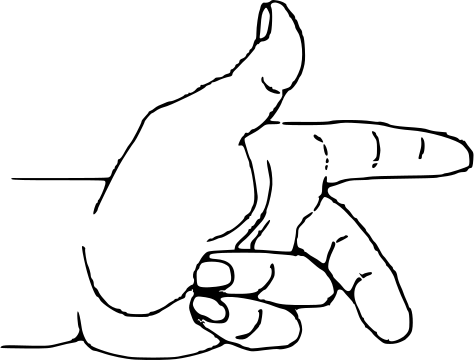
\includegraphics[width=4cm]{left-hand}};
                \coordinate (origin) at (0.45,0.2);

                \draw[ultra thick, ->, blue] (origin) -- ($(origin) + (0,2)$);
                \draw[ultra thick, ->, green] (origin) -- ($(origin) + (2,0)$);
                \draw[ultra thick, ->, red] (origin) -- ($(origin) + (1,-1.4)$);

                \node[below left=2.3 of origin] {\large \bf left hand!};
                \node[align=left,above left=0.7 of origin] {\textbf{Thumb}: \\
                direction of \\ conductor motion};

                \node[align=left,above right=0.5 of origin] {\textbf{Fore
                Finger}:\\ direction of fixed \\magnetic field (N to S)};

                \node[align=left,below right=of origin] {\textbf{Middle
                Finger}:\\ conventional current direction};
            \end{tikzpicture}
        }
    \end{center}




\end{frame}

{\fullbackground[scale=1]{ian-dc-motors-p6.pdf}
\begin{frame}{Using Fleming's Left Hand (Motor) Rule}
%
%The Left Hand Rule to determines the movement direction of conductor
%carrying current
%
%    \begin{center}
%        \resizebox{0.6\linewidth}{!}{
%            \begin{tikzpicture}[>=latex]
%                \node at (0,0) (hand) {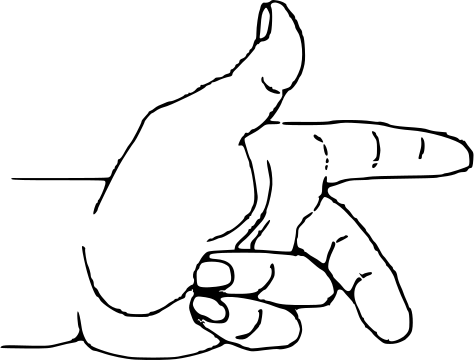
\includegraphics[width=4cm]{left-hand}};
%                \coordinate (origin) at (0.45,0.2);
%
%                \draw[ultra thick, ->, blue] (origin) -- ($(origin) + (0,2)$);
%                \draw[ultra thick, ->, green] (origin) -- ($(origin) + (2,0)$);
%                \draw[ultra thick, ->, red] (origin) -- ($(origin) + (1,-1.4)$);
%
%                \node[below left=2.3 of origin] {\large \bf left hand!};
%                \node[align=left,above left=0.7 of origin] {\textbf{Thumb}: \\
%                direction of \\ conductor motion};
%
%                \node[align=left,above right=0.5 of origin] {\textbf{Fore
%                Finger}:\\ direction of fixed \\magnetic field (N to S)};
%
%                \node[align=left,below right=of origin] {\textbf{Middle
%                Finger}:\\ conventional current direction};
%            \end{tikzpicture}
%        }
%        \includegraphics[width=0.6\linewidth]{image13}
%    \end{center}
%
\end{frame}
}

\begin{frame}{Single coil in magnetic field}

    \begin{center}
        \includegraphics[width=0.5\linewidth]{image15}
    \end{center}

\only<1>{
\begin{itemize}
    \item Current flow results in forces on sections that cut magnetic field
        $\vec{B}$
    \item Left section gets pushed up with force $\vec{F}$
    \item Right section gets pushed down with force $\vec{F}$ where
\[
    \vec{F} = \vec{I} \cdot L \times \vec{B}
\]

\end{itemize}
}

    \only<2>{

In practice the shaft torque of a DC motor is smaller than the
electromagnetic torque because of mechanical losses

\begin{itemize}
    \item Viscous friction will occur in the bearings
    \item Friction arises from the brushes rubbing on the commutator
    \item Air resistance will result in viscous friction due to rotation of the
    armature which may even include a cooling fan
\end{itemize}
}

\end{frame}

\begin{frame}{Cross-section of coil in magnetic field}

    \begin{center}
        \includegraphics<1>[width=0.8\linewidth]{image16-1}
        \includegraphics<2>[width=0.8\linewidth]{image16-2}
        \includegraphics<3->[width=0.8\linewidth]{image16-3}
    \end{center}

\only<3>{
If current $I$ flows through a coil of depth $L$ with magnetic field $B$,
the coil pivots and generates a torque $\tau$ given by:

\begin{equation*}
\begin{split}
\tau = 2 (\frac{d}{2}) \cdot F \cdot cos(\theta) &= d \cdot B \cdot I \cdot L \cdot cos(\theta) \\
                                                 &= d \cdot B \cdot I \cdot L
                                                 \text{\hspace{2em} when } \theta = 0^\circ \\
                                                 &= 0 \text{\hspace{2em} when } \theta = 90^\circ 
\end{split}
\end{equation*}


}

    \only<4>{

        \begin{columns}
            \begin{column}{0.7\linewidth}
                \small
        \begin{itemize}
            \item Moment arm = force $\times$ distance = torque
            \item As the coil rotates, moment arm is reduced and the torque decreases
            \item When the coil is horizontal it is at its maximum value
            \item When the coil is vertical it is zero
            \item NB: torque changes sign as we rotate 360°
        \end{itemize}
                
            \end{column}
            \begin{column}{0.3\linewidth}

    \resizebox{\linewidth}{!}{
        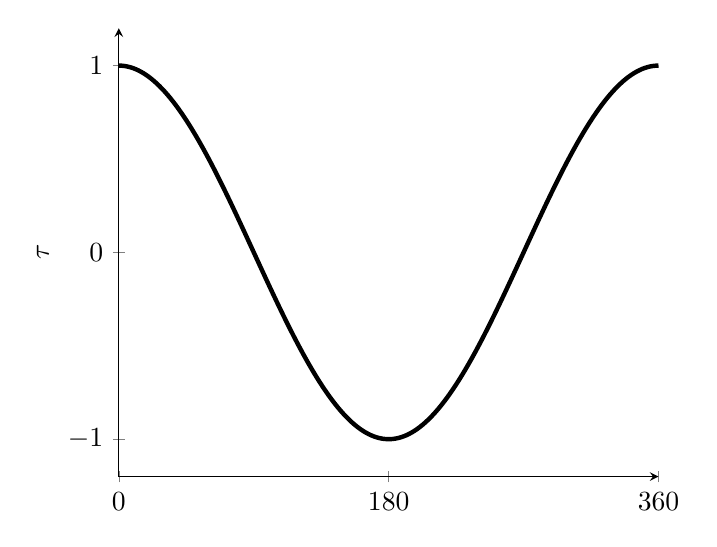
\begin{tikzpicture} 
            \begin{axis}[
                    xtick distance=180,
                    ytick distance=1,
                    no markers, samples=200,
                    axis x line=bottom,
                    axis y line=left,
                    domain=0:360,
                    ymin=-1.2, ymax=1.2,
                    ylabel=$\tau$
                ]
                \addplot[ultra thick] {cos(x)}; 
            \end{axis}
        \end{tikzpicture} 
    }
            \end{column}
        \end{columns}
}
\end{frame}

\begin{frame}{Commutation}

    \begin{columns}
        \begin{column}{0.3\linewidth}
            So coil of wire with fixed current direction has torque that changes
            sign as it rotates

            \vspace{2em}
            \resizebox{\linewidth}{!}{
                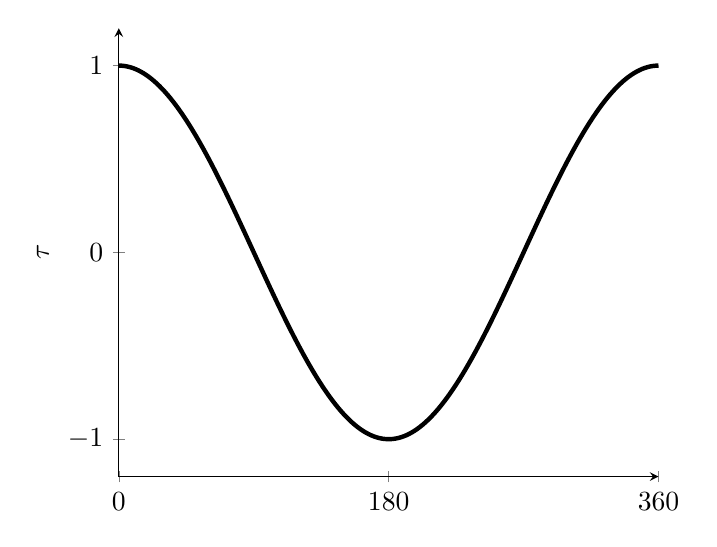
\begin{tikzpicture} 
                    \begin{axis}[
                            xtick distance=180,
                        ytick distance=1,
                        no markers, samples=200,
                        axis x line=bottom,
                        axis y line=left,
                        domain=0:360,
                        ymin=-1.2, ymax=1.2,
                        ylabel=$\tau$
                    ]
                        \addplot[ultra thick] {cos(x)}; 
                    \end{axis}
                \end{tikzpicture} 
            }
        \end{column}
        \begin{column}{0.3\linewidth}
            But we want torque always to be in the same direction!

            So use commutator to switch it!

            \begin{center}
                \includegraphics[width=1.2\columnwidth]{image22}
            \end{center}
        \end{column}
        \begin{column}{0.3\linewidth}

            Switching current direction before torque direction flips ensures
            that it is always in same direction
            
            \vspace{2em}
            \resizebox{\linewidth}{!}{
                \begin{tikzpicture} 
                    \begin{axis}[
                            xtick distance=180,
                        ytick distance=1,
                        no markers, samples=200,
                        axis x line=bottom,
                        axis y line=left,
                        domain=0:360,
                        ymin=-1.2, ymax=1.2,
                        ylabel=$\tau$
                    ]
                        \addplot[ultra thick] {abs(cos(x))}; 
                    \end{axis}
                \end{tikzpicture} 
            }
        \end{column}
    \end{columns}



\end{frame}

\begin{frame}{Precious metal commutators}

    \begin{columns}
        \begin{column}{0.6\linewidth}
            \begin{itemize}
                \item Well suited for smallest currents and~voltages
                \item Well suited for continuous operation
                \item Smaller motors
                \item Very low friction
                \item Low audible noise
                \item Low electromagnetic interference
                \item Cost effective
                \item Not suited for high current and peak currents
                \item Not suited for start-stop operation
            \end{itemize}

        \end{column}
        \begin{column}{0.4\linewidth}
            \begin{center}
                \resizebox{\linewidth}{!}{
                    \begin{tikzpicture}[>=latex]

                        \coordinate (anchor) at (-1.9,-0.1);
                            \node at (0,0) {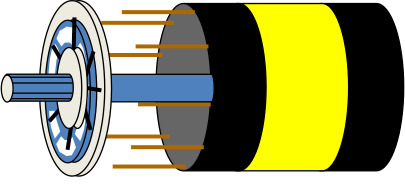
\includegraphics[width=\linewidth]{precious-metal-commutators}};
                            \node at (-0.2,-2) (caption) {\footnotesize silver commutator} edge[bend left,thick,->] (anchor);
                    \end{tikzpicture}
                }
            \end{center}
        \end{column}
    \end{columns}

\end{frame}

\begin{frame}{Carbon brush commutators}
    \begin{columns}
        \begin{column}{0.6\linewidth}

            Graphite brushes

            \begin{itemize}
                \item Well suited for high currents and peak currents
                \item Well suited for start-stop and reversing operation
                \item Larger motors ($>$ approx. 10 W)
                \item Higher friction
                \item Higher no-load current
                \item Not suited for small currents
                \item Higher audible noise
                \item Higher electromagnetic emissions
                \item Higher costs
            \end{itemize}

        \end{column}
        \begin{column}{0.4\linewidth}

            \begin{center}
                \resizebox{\linewidth}{!}{
                    \begin{tikzpicture}[>=latex]

                        \coordinate (anchor) at (-1.5,0);
                            \node at (0,0) {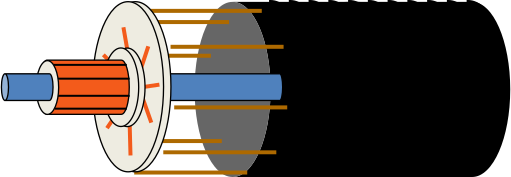
\includegraphics[width=\linewidth]{carbon-brush-commutators}};
                            \node at (0,-1.5) (caption) {\footnotesize copper
                            commutator} edge[bend left,thick,->] (anchor);
                    \end{tikzpicture}
                }

                \vspace{2em}
                \includegraphics[width=0.8\linewidth]{image23}
            \end{center}
        \end{column}
    \end{columns}


\end{frame}

{\fullbackground[scale=0.9,page=21]{../part1/figs/ian-sensors.pdf}
    \begin{frame}{Electronic commutation systems}
    \note {
In this third part of the presentation we would like to understand the electronic commutation.
There are different systems. maxon uses the following three :

- Block commutation with or without Hall sensors
- Sinusoidal commutation.

As you can see the different maxon controller families perform different commutation types.

Common to all these systems is that they should apply the current in a way, that the generated torque is as high as possible. As we have learned this is achieved by a perpendicular orientation of the magnetic fields of permanent magnet and winding. We have seen as well that we need to know the orientation of the permanent magnet to achieve this.

We start with block commutation with Hall sensor position feedback. That's the standard commutation type. Once we have understood this the two other commutation schemes are easily derived from it.
    }
    \end{frame}
}

{\fullbackground[scale=0.9,page=22]{../part1/figs/ian-sensors.pdf}
    \begin{frame}{Block commutation}

\note{
First we have to look at the Hall sensor feedback signals. Again we do this
based on the simplest design, the slotless maxon EC motor with 1 pole pair.

In the back of the motor there are three Hall sensor mounted on the PCB at an
angle of 120°. The Hall sensor detect the magnetic poles of the control magnet
which is mounted on the shaft. The control magnet exhibits the same two
magnetic poles in the same orientation as the power magnet. (Basically the Hall
sensors could monitor the power magnet directly but the control magnet offers
two advantages: The magnetic transitions between north and south pole are more
precisely defined. And an angular misalignment and tolerances between the
relative position of winding and Hall sensors can be adjusted.)

The digital Hall sensors used probe the direction of the magnetic field. They
generates a high output signal (5V) if the north pole of the control magnet is
close to them. A south pole produces a low level (Gnd).

The actual position of the control magnet in the diagram generates the
following signals:

- The blue Hall sensor sees the north pole. Thus the signal output level is
high and will remain high for the next 120°.
- The green Hall sensor is close to the south pole. The output level is low for
the next 60°. Then the north pole approaches and the output signal will switch
to a high state.
- The red Hall sensor has just switched from high to low where the signal level
will stay for the next half a turn.

The combination of the three Hall sensor signals is unique for each 60° of
rotation. Looking at these signals allows to know the rotor position within
60°. That exactly what we need for commutation. Remember there were 6 different
ways of current flow through the motor at a commutation angle of 60°.

The next slide shows how the complete block commutation system works.
}
    \end{frame}
}

{\fullbackground[scale=0.9,page=23]{../part1/figs/ian-sensors.pdf}
    \begin{frame}{Components of an EC drive system}
\note{
Let's first look at an EC drive system in general.

The three phases of the EC motor cannot be connected directly to a DC power
supply. The voltage needs to be switched in a sequence. This is done by the
electronic commutation. For the correct switching the electronics needs rotor
position information from the motor. This information is usually provided by
the Hall sensors.

An EC motor cannot operate on its own: It's always the combination of motor and
electronics commutation that makes the full drive.


For more sophisticated commutation and precise motor control, e.g. at very low
speeds, the use of an encoder feedback might be necessary. Often the
electronics not only performs the commutation but at the same time can be used
to control speed or position.
}
    \end{frame}
}


\begin{frame}{DC Motor Torque Ripple}

    \begin{center}
        \includegraphics[height=0.4\paperheight]{image24}\hspace{1em}
        \video[1]{0.35\linewidth}{part2/figs/torque-ripple.mp4?autostart&loop}
    \end{center}

\begin{itemize}
\item With single coil the torque still drops to zero when the coil is
  vertical
\item This fluctuation is known as torque ripple
\item However with torque always in same direction coil will now rotate
  continuously
\end{itemize}

\end{frame}

\begin{frame}{Multiple coils reduces torque ripple}

    \begin{columns}
        \begin{column}{0.5\linewidth}
            \begin{center}
                \includegraphics[width=\linewidth]{image26}

                \vspace{2em}

                \footnotesize Overall torque summed from both coils

                \includegraphics[width=\linewidth]{image26-2}

            \end{center}
        \end{column}
        \begin{column}{0.5\linewidth}

            \begin{center}
                \includegraphics[width=0.8\linewidth]{image27}

                Typical small armature with multiple multi-turn coils
            \end{center}
        \end{column}
    \end{columns}


\end{frame}

\begin{frame}{DC motor as an energy converter}


\begin{itemize}

\item Converts electrical energy into mechanical energy + heat
\item Electrical power in = voltage $\times$ current
\item Mechanical power out = Speed ($rad \cdot s^{-1}$) $\times$ torque ($N\cdot m$)
\end{itemize}

    \begin{columns}
        \begin{column}{0.7\linewidth}
    \begin{center}
        \resizebox{0.9\linewidth}{!}{
            \begin{tikzpicture}[>=latex]

                \node at (0,0) (motor) {\includegraphics[width=3cm]{maxon}};
                \node[below left=0.5 of motor] (pmech) {$P_{mech}=2\pi\frac{n}{60}\cdot \tau$};
                \node[above right=0.5 of motor] (pel) {$P_{el}=V \cdot I$};
                \node[below right=0.5 of motor] (pr) {$P_{r}=R \cdot I^2$};
                \draw[ultra thick, red,->] (motor) -- (pmech);
                \draw[ultra thick, red,->] (pel) -- (motor);
                \draw[ultra thick, orange,->] (motor) -- (pr);
            \end{tikzpicture}
        }

    \[
        P_{el} = P_{mech} + P_{r} = V\cdot I = 2\pi\frac{n}{60}\cdot \tau + I^2 R
    \]
    \end{center}

        \end{column}
        \begin{column}{0.3\linewidth}
    \footnotesize
    where:

        $\tau$ = torque;
        
        $N$ = rotation speed in rpm;
        
        $I$ = input current;
        
        $V$ = applied voltage
            
        \end{column}
    \end{columns}

\note{

In a very general frame motors can be considered as energy converters.
DC motors convert the electrical input power (DC voltage V and current
I) into mechanical output power consisting of angular speed ω and torque
M. Engineers prefer to use rotational speed n measured in rpm instead of
rad/s; that's why there is a factor of π/30 to get the unit of power
right in Watts.

The theory described in this presentation applies to any DC motor, in
particular to the maxon DC motor and the brushless maxon EC motor.
}

\end{frame}

\section[Construction]{DC motor construction}

\begin{frame}{Basic parts of a brushed DC motor}

\begin{columns}
    \footnotesize
    \begin{column}{0.5\linewidth}
    \begin{itemize}
        \item Bearings are mounted each end of the output shaft
        \item Housing provides support for the bearings and holds the stator magnets
        \item It also provides protection and mechanical attachment
        \item Armature may have skewed coil slots to reduce cogging
    \end{itemize}

    \resizebox{\columnwidth}{!}{
    \begin{tikzpicture}[>=latex]
        \node at (0,0) {\includegraphics[width=0.9\columnwidth]{image39}};
        \node at (-2,1.5) {\footnotesize brushes} edge[bend left,thick,->] (-1.2,0.5);
        \node at (-0.5,1.5) {\footnotesize housing} edge[bend left,thick,->] (0.5, 1);
        \node at (2,1.5) {\footnotesize bearings} edge[bend left,thick,->] (1.7, 0.7);
        \node at (0,-1.3) {\footnotesize commutator} edge[bend left,thick,->] (0,0);
        \node at (2,-1) {\footnotesize laminated iron core} edge[bend left,thick,->] (1,0);
    \end{tikzpicture}
    }


    \end{column}
    \begin{column}{0.5\linewidth}
    \begin{itemize}
        \item Stator magnets generate magnetic field so current in coils generate
        toque
        \item Armature rotor consists of laminated iron core wrapped with coils to
        give mow reluctance but avoid eddy current
        \item Commutator used so switch current direction and permit continuous
        rotation
        \item Brushes provide contact to commutator
    \end{itemize}


    \resizebox{\columnwidth}{!}{
        \begin{tikzpicture}[>=latex]
            \node at (0,0) {\includegraphics[width=0.9\columnwidth]{image38}};
        \end{tikzpicture}
    }


    \end{column}
\end{columns}
\end{frame}

\imageframe[color=black,caption=Typical example of commutated armature]{image40}


\begin{frame}{Coreless Maxon DC motor (RE 35)}

    \resizebox{\columnwidth}{!}{
        \begin{tikzpicture}[>=latex]
            \node at (0,0) {\includegraphics[width=0.9\columnwidth]{image41}};
            \node at (-4.7,-1.5) {\footnotesize press ring} edge[thick,->] (-4.5,-0.9);
            \node at (-3.8,-2) {\footnotesize ball bearing} edge[thick,->] (-3.8,-1.1);
            \node at (-4,0.3) {\footnotesize el. connections};
            \node at (-3,1) {\footnotesize brushes} edge[bend left,thick,->] (-1.8,0);
            \node at (-1.5,-2) {\footnotesize commutator} edge[bend left,thick,->] (-1.2,-0.2);
            \node at (-2,1.5) {\footnotesize commutator plate} edge[bend left,thick,->] (-1.2,0.5);
            \node at (-1,2) {\footnotesize self supporting winding} edge[bend left,thick,->] (-0.5,0.6);
            \node at (0.5,1.5) {\footnotesize shaft} edge[thick,->] (0.5,0);
            \node[minimum width=2cm,align=center] at (1,-1.5) {\footnotesize permanent magnet\\ \footnotesize(in the centre)} edge[bend right,thick,->] (2,-0.2);
            \node[minimum width=2cm,align=center]  at (3,-2) {\footnotesize housing\\ \footnotesize (magnetic return)} edge[bend right,thick,->] (2.5,-0.5);
            \node at (4,-0.8) {\footnotesize flange} edge[bend right,thick,->] (3.5,-0.2);
            \node at (3,2) {\footnotesize ball bearing} edge[bend left,thick,->] (3.8,0.9);
            \node at (3.6,2.5) {\footnotesize press ring} edge[bend left,thick,->] (4.5,0.9);

            %\grid{}
        \end{tikzpicture}
    }



\note{
This picture shows a coreless maxon DC motor. We recognize the same
three subassemblies as with the conventional motor.

The \textbf{stator} consists of the permanent magnet at the centre (here
shown in green), of the housing (again serving as the magnetic return)
and of the mounting flange.

The \textbf{rotor} with winding and commutator. The winding is connected
to the shaft by the so called commutator plate. In this example the
shaft is supported in the stator by ball bearings. The shape of the
rotor reminds of a Xmas bell; that's why it is sometimes called ``bell
shaped'' armature. The winding moves in the air gap between magnet and
housing.

The \textbf{brush system} here with graphite brushes in red and with the
electrical motor connections.

The next slides show the advantages of a ironless motor design.
}

\end{frame}

\begin{frame}{Magnetic circuit of the Maxon Stator}

    \resizebox{\linewidth}{!}{
        \begin{tikzpicture}[>=latex]
            \node at (0,0) {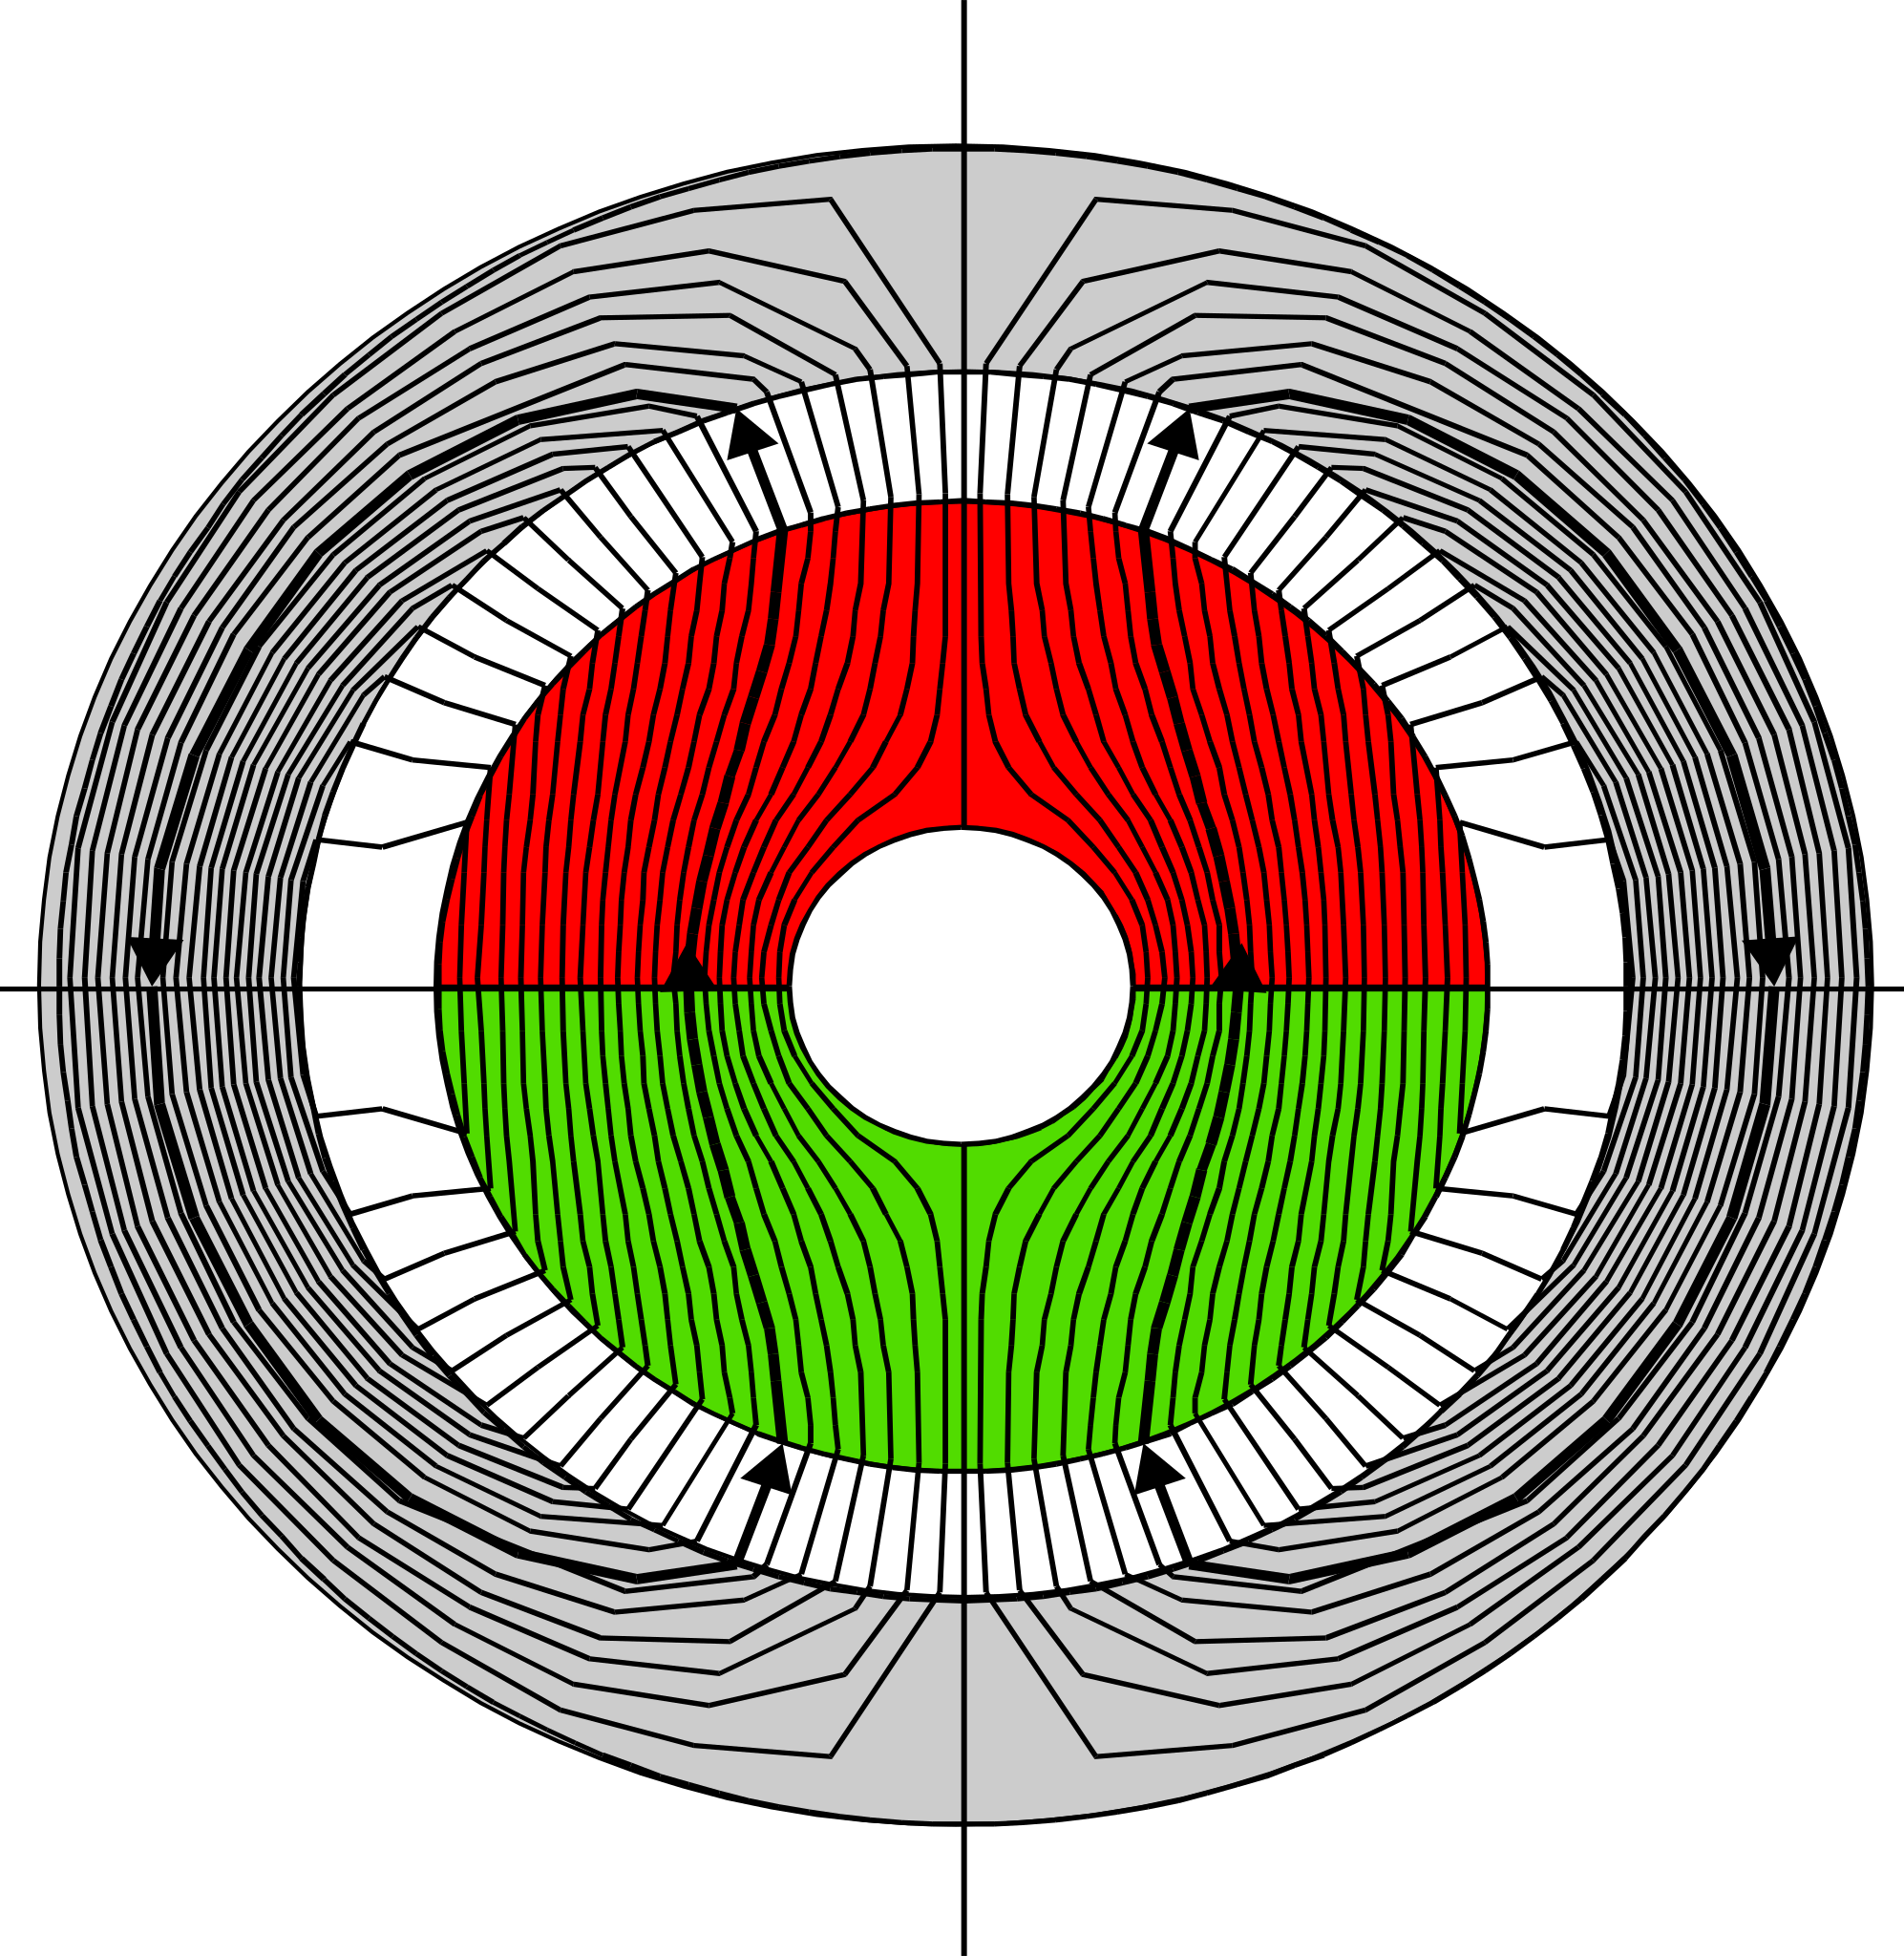
\includegraphics[width=0.5\linewidth]{maxon_stator}};

            \node[minimum width=2cm,align=left,anchor=west] at (3,2) {\footnotesize \textbf{Housing}\\ magnetic return path made\\ of magnetic steel (iron)\\ guides magnetic field} edge[bend right,thick,->] (1.5,1.5);
            \node[minimum width=2cm,align=left,anchor=west]  at (3.5,0) {\footnotesize \textbf{Air gap}\\ the larger the air gap, \\the weaker the magnetic field} edge[thick,->] (1.8,0.5);
            \node[minimum width=2cm,align=left,anchor=west]  at (3,-2) {\footnotesize \textbf{Permanent magnet}\\ produces the magnetic field \\with north and south pole \\on opposite sides} edge[bend left,thick,->] (0.5,-0.5);
            %\grid{}
        \end{tikzpicture}
    }

\note{

After this introduction let's now consider the magnetic circuit in the
stator in more detail.

This slides shows a cross section of the stator.

In the centre we have the \textbf{permanent magnet}. It is diametrically
magnetized, the north pole being colored in red, the south pole in
green. The bore in the middle serves for the motor shaft.

The \textbf{magnetic field lines} leave the magnet at the north pole and
enter the magnet at the south pole. Magnetic field lines - more exactly
the magnetic induction B - are closed lines and must be guided back from
the north to the south pole. That's the duty of the housing which is
made of a magnetically conducting material. That's why the housing is
also called \textbf{magnetic return}.

Between the permanent magnet and the magnetic return the field lines
point in radial direction in the \textbf{air gap}. The goal of this
arrangement is to create an magnetic field as strong as possible in the
air gap in order for the winding to produce as much force as possible.
Air is a bad magnetic conductor and the larger the air gap the smaller
the magnetic flux that can be built. That's why the air gap should be as
narrow as possible. However in a narrow air gap there is room for only a
thin walled winding. The current density is small and so is the produced
force. We see that finding the right dimensions for the air gap is a
classic optimization problem depending strongly on the properties of the
permanent magnet.

In short: We have a configuration producing a magnetic field in the air
gap which points from bottom to top in this representation.

}

\end{frame}

\begin{frame}{Maxon DC motors versus conventional motors}

    \begin{columns}
        \begin{column}{0.5\linewidth}

            \begin{center}
                \includegraphics[width=0.8\columnwidth]{image46}
            \end{center}

Conventional motor with rotating magnet and iron core

\begin{itemize}

\item Detent torque (cogging)
\item Inefficient, iron core losses
\item Large physical size
\item High inertia
\end{itemize}

        \end{column}
        \begin{column}{0.5\linewidth}

            \begin{center}
                \includegraphics[width=0.8\columnwidth]{image45}
            \end{center}


Maxon motor with stationary magnet and special winding

\begin{itemize}
\item Smooth
\item Linear Characteristic
\item Efficient
\item Responsive
\item Powerful
\end{itemize}

        \end{column}
    \end{columns}

\end{frame}

\begin{frame}{Advantage of coreless armature}

\begin{columns}
    \begin{column}{0.6\linewidth}

\begin{itemize}

\item No iron core - no iron losses
\item Constantly impressed magnetization
\item High efficiency, up to over 90\%
\item No saturation effects in the iron core
\item Even at the highest currents the produced torque is proportional to
  the motor current
\item Stronger magnets = stronger motors
\end{itemize}

    \end{column}
    \begin{column}{0.4\linewidth}

        \begin{center}
            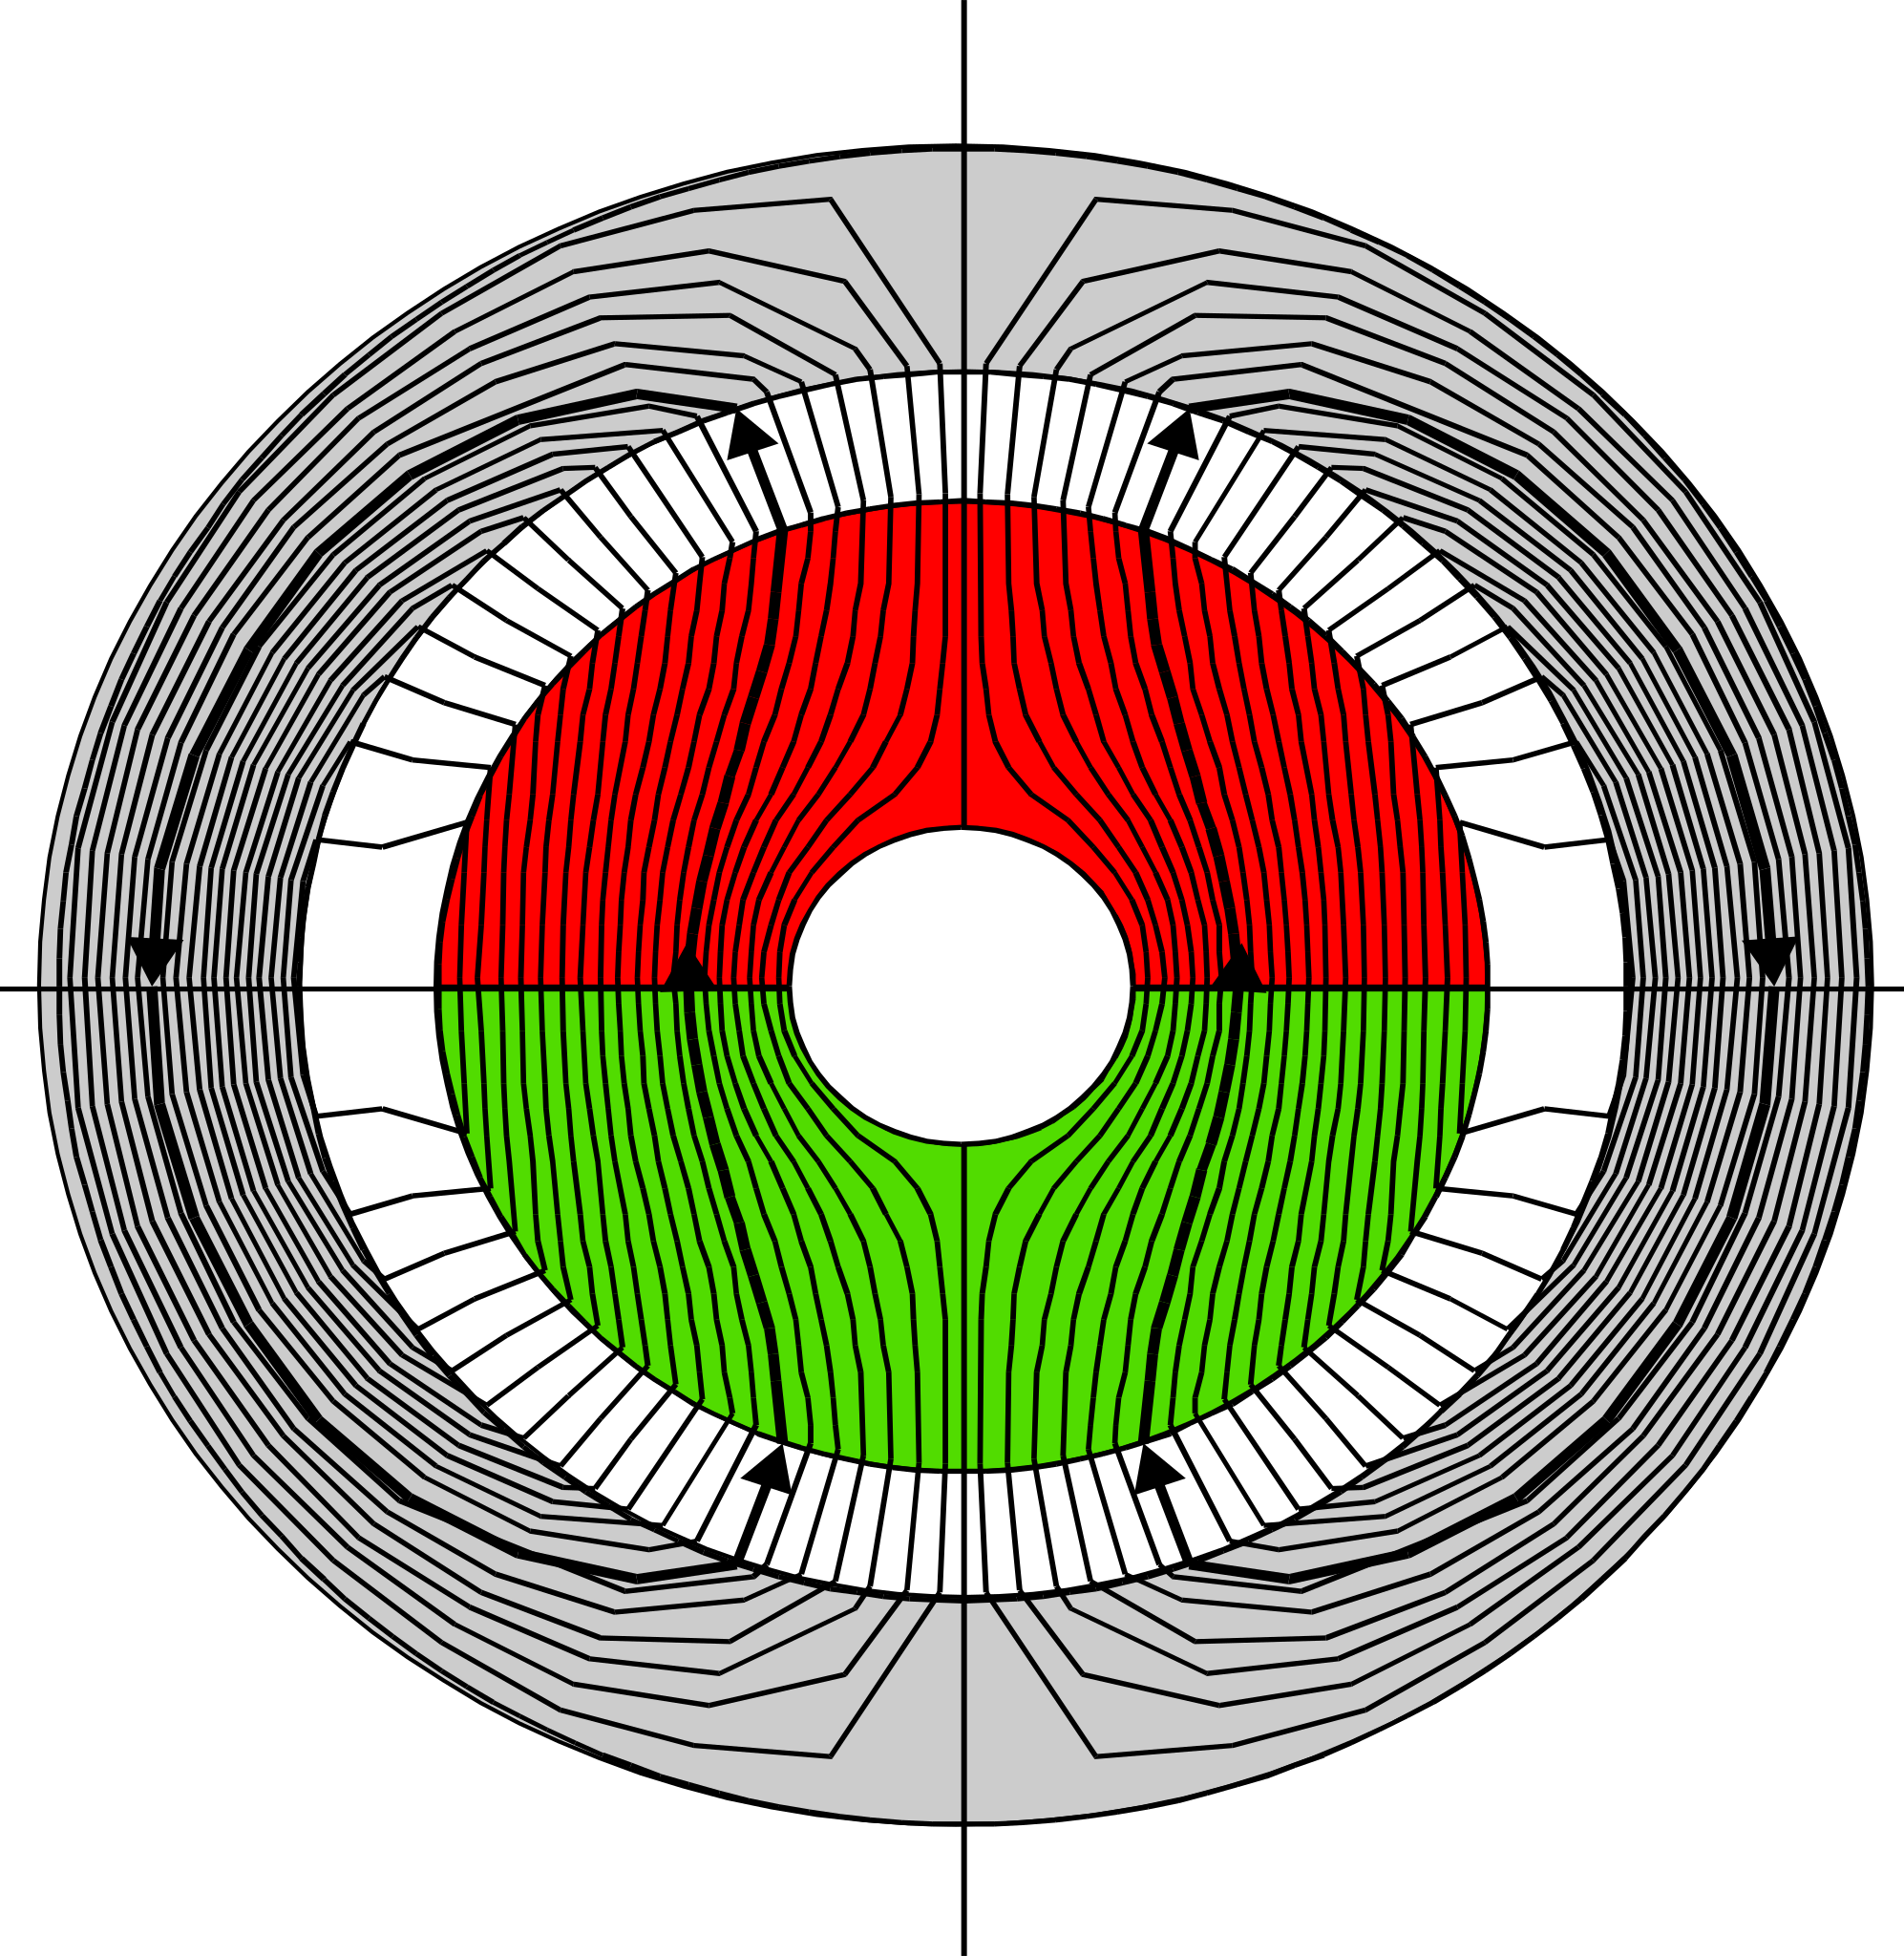
\includegraphics[width=0.8\columnwidth]{maxon_stator}
        \end{center}
    \end{column}
\end{columns}

    \note{

Coreless DC motors have \textbf{no iron losses}.

In a conventional design the iron core permanently changes its
magnetization. This consumes energy because the magnetic hysteresis loop
must be run through at each shaft rotation. Additionally these flux
variations induce Eddy currents in the iron core resulting in power
losses that grow with the square of the motor speed.

By contrast, in a coreless motor the Magnetization is permanently
impressed and constant. (The influence of the magnetic field of the
winding can be neglected in a first approximation.) Hence there are no
iron losses. As a result, the power losses are smaller, the
\textbf{efficiency is higher} and the \textbf{no-load current is lower}.

In an ironless design \textbf{no saturation} at the narrow parts of the
iron core (at the base of the teeth) can occur. Hence the produced
torque remains \textbf{exactly proportional} to the motor current and
one can use the strongest permanent magnets without being limited by the
maximum magnetic flux in the iron core. Improvements in magnet
technology lead to \textbf{stronger motors}.

}

\end{frame}

\begin{frame}{2 and 4 pole motors}

    We don't need to limit number of poles to two

    \begin{columns}
        \begin{column}{0.5\linewidth}
            \begin{center}
                \includegraphics[height=0.5\paperheight]{image48}

                \textbf{2 pole motors}
            \end{center}
        \end{column}
        \begin{column}{0.5\linewidth}

            \begin{center}
                \includegraphics[height=0.5\paperheight]{image49}

                \textbf{4 pole motors}
            \end{center}
        \end{column}
    \end{columns}


\end{frame}



%%%%%%%%%%%%%%%%%%%%%%%%%%%%%%%%%%%%%%%%%%%%%%%%%%%%%%%%
%%%%%%%%%%%%%%%%%%%%%%%%%%%%%%%%%%%%%%%%%%%%%%%%%%%%%%%%
\miniframesoff
\begin{frame}{}
    \begin{center}
        \Large
        That's all, folks!\\[2em]

        \normalsize
        \textbf{Questions}:\\
        Portland Square B316 or \url{severin.lemaignan@plymouth.ac.uk} \\[1em]

        \textbf{Slides}:\\
        \href{https://github.com/severin-lemaignan/module-introduction-sensors-actuators}{\small
        github.com/severin-lemaignan/module-introduction-sensors-actuators} \\

        ...or the DLE!


    \end{center}
\end{frame}




\end{document}
